\begin{figure*}[t!]
\centering
\begin{tabular}{ccc}
\begin{minipage}{0.46\textwidth}
\centering
\begin{tabular}{|c|}
\hline
\indent\vspace{-0.0cm}\\
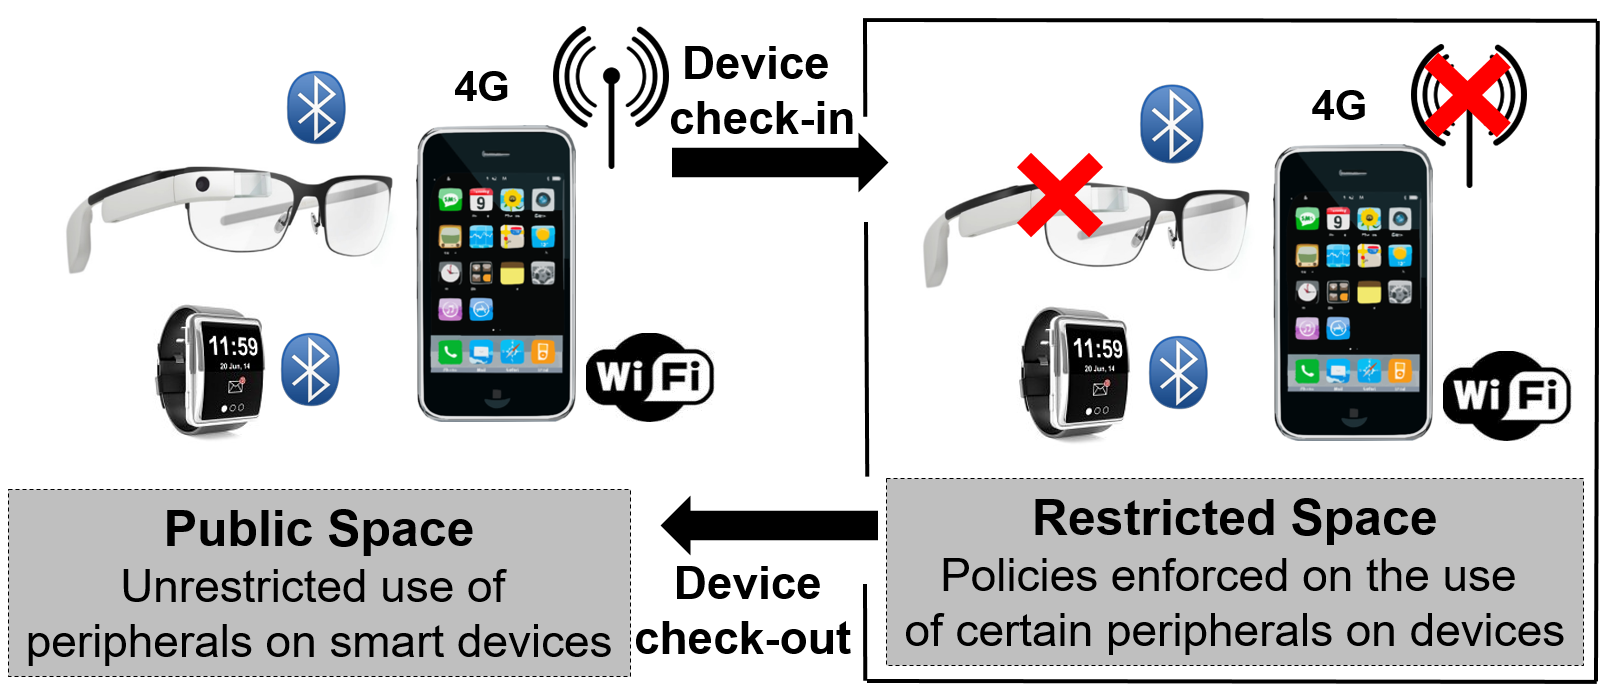
\includegraphics[keepaspectratio=true,width=0.95\textwidth]{figures/restricted-space.png}\\
\multicolumn{1}{|p{0.98\textwidth}|}
{\small {\bf Restricted space model.} Guests ``check-in'' their personal
devices when entering restricted spaces. During check-in, hosts inspect,
analyze and modify the configurations of these devices in accordance with their
usage policies. In this example, the host restricts the use of the camera on
the smart glass, and the 4G data interface on the smart phone. However, the
glass and watch can continue to use Bluetooth pairing, while the phone can
connect to the host's access points using WiFi.  When guests leave the
restricted space, they ``check-out'' their devices, restoring them to their
original configurations.}\\
\hline
\end{tabular}
\end{minipage} & & 
\begin{minipage}{0.46\textwidth}
\centering
\begin{tabular}{|c|}
\hline
\indent\vspace{-0.2cm}\\
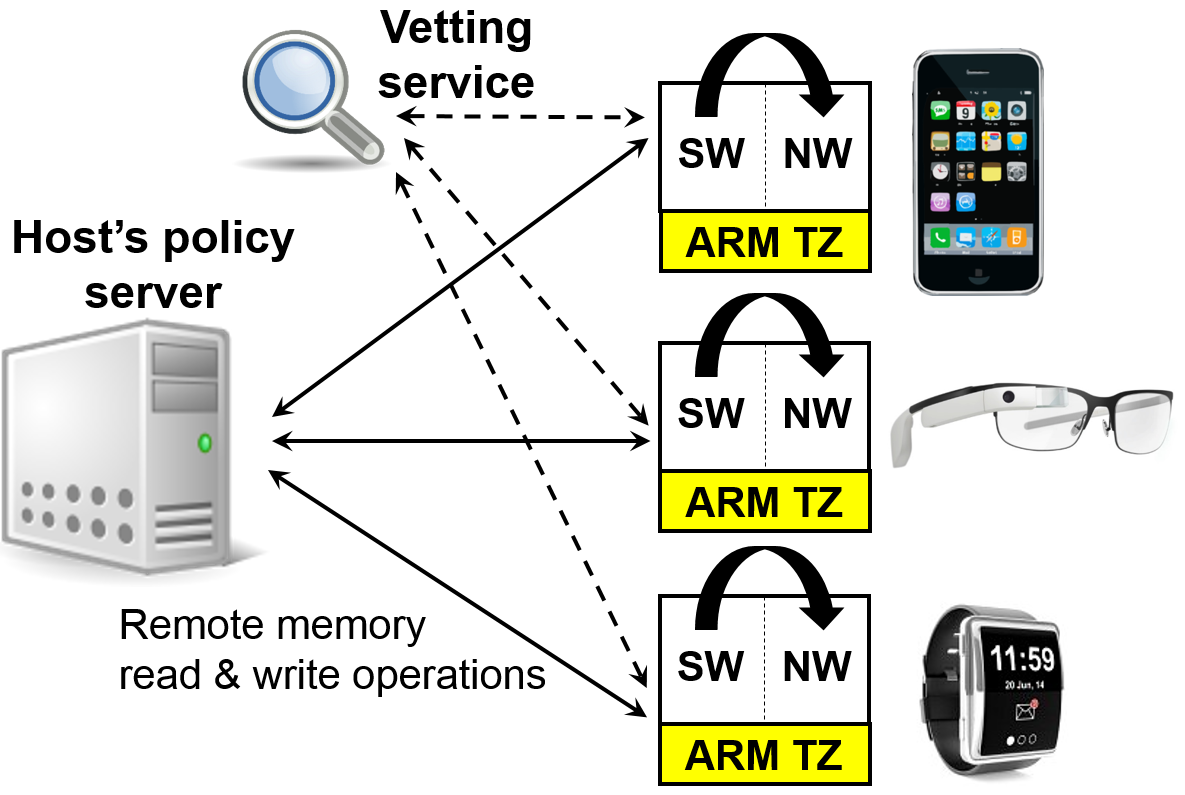
\includegraphics[keepaspectratio=true,width=0.90\textwidth]{figures/host-guest.png}\\
\indent\vspace{-0.5cm}\\
\multicolumn{1}{|p{0.98\textwidth}|}
{\small {\bf Guest device setup.} Guest devices are equipped with ARM TrustZone
and execute components of the policy enforcement mechanism in the secure world
(SW). The details of this mechanism appear in \sectref{section:mechanism}.  At
check-in, the host's policy server leverages the secure world to remotely
inspect and modify normal world (NW) memory.}\\
\hline
\end{tabular}
\end{minipage}
\end{tabular}
%\indent\vspace{-0.5cm}
\mycaption{An overview of the entities of our restricted space model and the
setup of guest devices.}
{\label{figure:restrictedspaces}}
\end{figure*}

\mysection{Restricted Spaces}
\label{section:usagemodel}

We provide an overview of the restricted space model, motivate some features of
our enforcement mechanism, and describe our threat model. Because our mechanism
relies on the ARM TrustZone, we begin by introducing its features.

\subsection{Background on the ARM TrustZone}
\label{section:armback}

The TrustZone is a set of security enhancements to chipsets based on the ARM
architecture. These enhancements cover the processor, memory and peripherals.
With TrustZone, the processor executes instructions in one of two security
modes at any given time, a \textit{normal world} and a \textit{secure world}. A
third \textit{monitor mode} facilitates switching between the normal and the
secure worlds.  The secure and normal worlds have their own address spaces and
different privileges.  The processor switches from the normal world to the
secure world via an instruction called the secure monitor call (\textsf{smc}).
When an \textsf{smc} instruction is invoked from the normal world, the
processor context switches to the secure world (via monitor mode) and freezes
execution of the normal world.

The ARM TrustZone partitions memory into two portions, with one portion
being exclusively reserved for the secure world. It also allows individual
peripherals to be assigned to the secure world.  For these peripherals,
hardware interrupts are directly routed to and handled by the secure world.
While the normal world cannot access peripherals or memory assigned to the
secure world, the secure world enjoys unrestricted access to all memory and
peripherals on the device. It can therefore access the code and data of the
normal world. The secure world can execute arbitrary software, ranging from
simple applications to an entire operating system (OS).
%
% NOT the CPU state. Registers are "banked", and only monitor mode can view
% them all.

A device with ARM TrustZone boots up in the secure world. After the secure
world has initialized, it switches to the normal world and boots the OS there.
Most TrustZone-enabled devices are configured to execute a \textit{secure boot}
sequence that incorporates cryptographic checks into the secure world boot
process~\cite[\S5.2.2]{armtz}. For example, the device vendor signs the code
with its private key, and the vendor's code in the boot ROM verifies this
signature using the vendor's public key. These checks ensure that the integrity
of the boot-time code in the secure world has not been compromised, \eg~by
reflashing the image on persistent storage. Most vendors lock down the secure
world via secure boot, thereby ensuring that it cannot be modified by
end-users. This feature allows hosts to trust software executing in the secure
world and treat it as part of the trusted computing base (TCB). In this paper,
we assume that guest devices use secure boot.

\subsection{Entering and Exiting Restricted Spaces}
\label{section:usagemodel:checkin}

\myparagraph{Check-in} When a guest enters a restricted space, he checks in
each of his devices during entry (\figref{figure:restrictedspaces}).  During
check-in, the guest device communicates with the host's policy server for the
following tasks:

\begin{mylist}
%
\item \emphitem{Authentication.} The first step is for the host and the guest to
mutually identify each other. We assume that both the guest and the host have
cryptographic credentials (\eg~public/private key pairs) that are validated
via a trusted third party, such as a certifying authority. The host and the
guest mutually authenticate each other's credentials in the standard way, as is
done during SSL/TLS handshakes.

The host's policies are enforced by a mechanism that executes in the secure
world of the guest device. We rely on TrustZone's secure boot sequence to
prevent unauthorized modifications to this code. Note that the end-user's usual
work environment on the device, \eg~the traditional Android, iOS or Windows
environment with apps, executes in the normal world (and is untrusted). We
expect the secure world software running the mechanisms proposed in this paper
to be created and distributed by trusted entities, such as device vendors, and
execute in isolation on guest devices.

\item \emphitem{Host remotely reads guest state.} The host requests the guest
device for a snapshot of its normal world memory and CPU register state. The
secure world on the device fulfills this request (after it has been cleared by
the vetting service) and sends it to the host. The secure world also sends a
cryptographic checksum of this data to prevent unauthorized modifications
during transit.

The host uses raw memory pages from the device in two ways. First, it scans
memory pages to ensure that the normal world kernel is free of malicious
software. A clean normal world kernel can bootstrap additional user-level
security mechanisms, \eg~an antivirus to detect malicious user-level apps.
Second, it extracts the normal world's configuration information. This includes
the kernel version, the list of peripherals supported, memory addresses of
various device drivers for peripherals and the state of these peripherals
\eg~whether a certain peripheral is enabled and its settings. The host can also
checkpoint the configuration for restoration at check-out. 

\addtext{Task 7}{The host terminates check-in at this point if it finds that
the guest device is malicious or runs a kernel version that it cannot
reconfigure. The action that the host takes depends upon the specific setting.
For example, in a federal building, the device owner may be asked to quarantine
the device outside the restricted space or enclose it in a physically-secured
Faraday cage. In less stringent settings, the host may blacklist the device's
MAC address and prevent it from connecting to any local resources in the
restricted space. Note that benign end-users may not have willingly installed
malware on their devices. A failed check-in has the desirable side-effect of
allowing such end-users to detect that their device is infected.}

\item \emphitem{Host remotely modifies guest state.} The host modifies the guest
device to conform to its restricted usage policies.  The host's restrictions on
a guest device depend on what it perceives as potential risks.  Cameras and
microphones on guest devices are perhaps the most obvious ways to violate the
host's confidentiality because they can be used to photograph confidential
documents or record sensitive meetings. Networking and storage peripherals such
as WiFi, 3G/4G, Bluetooth and detachable storage dongles can work in concert
with other peripherals to exfiltrate sensitive information. Dually, guest
devices can also be used to infiltrate unauthorized information into restricted
spaces, \eg~students can cheat on exams by using their devices to communicate
with the outside world.

The host controls peripherals on guest devices by creating a set of updates to
the device's normal world memory and requesting the secure world to apply them.
For example, one way to disable a peripheral is to unlink its driver from the
device's normal world kernel (details in \sectref{section:policy}).  The secure
world applies these updates after using the vetting service to ensure the
safety of the requested updates.

We assume that it is the host's responsibility to ensure that the memory
modifications are not easily bypassable. For example, they may be undone if the
user of the guest device directly modifies kernel memory, \eg~by dynamically
loading kernel modules or using \textsf{/dev/kmem} in the normal world. The
host must inspect the guest device's snapshot for configurations that lead to
such attacks, and disallow the use of such devices in the restricted space.

In steps \circtwo\ and \circthree, the secure world performs the host's read
and write operations only if they are approved by the vetting service. Guests
configure the vetting service to suit their security and privacy goals. If the
vetting service deems an operation unsafe, device check-in is aborted and the
device is left unmodified. The guest cannot use the device in the restricted
space because its security and privacy goals conflict with the host's usage
policies.

\item \emphitem{Host obtains verification token from guest.} After the guest
device state has been modified, its secure world produces a verification token
to be transmitted to the host. The verification token is a cryptographic
checksum over the memory locations that were modified. The token is unforgeable
in that only the secure world can re-create its value as long as the host's
memory updates have not been altered, and any malicious attempts to modify the
token can be detected by the secure world and the host.

\addtext{Task 5}{The check-in steps above bear some resemblance to TPM-based
software attestation protocols developed in the trusted computing
community~\cite{Sailer04}. Like TPM measurements, which attest the software
stack or properties of dynamic data structures~\cite{sadeghi:isc08},
verification tokens attest that a guest device's state complies with the host's
policies. Both TPM measurements and verification tokens are grounded in a
hardware root of trust.  However, unlike traditional software attestation,
which has largely been restricted to passive checks of a remote machine's
state, verification tokens attest to the integrity of the host's remote
modifications of the guest device.}

\addtext{Task 1}{Like in software attestation, a correct verification token
attests the state of the guest device only at the instant at which it was
produced by the secure world. To ensure that the guest device remains
policy-compliant, the host can request the device to send it the verification
token at any point when the device is in the restricted space.} 
The secure world on the device computes this token afresh, and transmits it to
the host,\footnote{This assumes that the host's policy still allows
communication between the host and the guest. If all of the guest's peripherals
are disabled, the host must physically access the guest to visually obtain the
fresh token.} which compares this freshly-computed token with the one obtained
during check-in. It uses this comparison to ensure that the guest has not
altered the normal world memory updates from the previous step. The
verification token incorporates a host-supplied challenge to ensure that the
guest device cannot simply replay old tokens. 
\addtext{Task 1}{As we demonstrate in \sectref{section:evaluation},
verification tokens are only a few hundred bytes in size and can be computed by
the secure world in just a few milliseconds. Thus, hosts can request guest
devices to send verification tokens at frequent intervals, thereby increasing
confidence that the guest device was continuously policy-compliant.}

The verification token is ephemeral, and can be computed afresh by the guest
only within an expiration period. The token expires upon device check-out or if
the device is powered off, thereby ensuring that end-users cannot undo the
host's memory updates by simply rebooting the device.  In
\sectref{section:mechanism:REMsuspend}, we describe
\textit{\underline{re}stricted space-\underline{m}ode (REM) suspend}, a special
protocol that suspends the device while allowing the verification token and the
host's memory updates to persist.
%
\end{mylist}

\myparagraph{Check-out} Once checked-in, the guest device are free to avail of
the facilities of the restricted space under the policies of the host. For
example, in \figref{figure:restrictedspaces}, the smart glass and watch can
pair with the smart phone via Bluetooth, while the smart phone can use the
host's WiFi access point. When the guest checks-out, two tasks must be
accomplished:
%
\begin{mylist}
%
\item \emphitem{Host checks guest state.} The host requests the guest to send
the verification token to ensure that the device is policy-compliant. The token
may not match the value obtained from the device at check-in if the host's
memory modifications have been maliciously altered or if the end-user chose to
consciously bypass REM-suspend and reboot the device.  It is not possible to
differentiate between these cases, and the host's policy to deal with
mismatches depends upon the sensitivity of the restricted environment. For
example, in a federal setting, detailed device forensics may be necessary. As
previously discussed, hosts can request the verification token from the device
at any time when it is in the restricted space. Hosts use this feature to
frequently check the verification token to narrow the timeframe of the
violation.

\item \emphitem{Restoring guest state.} To restore the state of the device, the
end-user simply performs a traditional device reboot. The host only modifies
the memory of the device, and not persistent storage. Rebooting therefore
undoes all the memory modifications performed by the host and boots the device
from an unmodified version of the kernel in persistent storage. Alternatively,
the host can restore the state of the device's peripherals from a checkpoint
created at check-in. The main challenge here is to ensure consistency between
the state of a peripheral and the view of the peripheral from the perspective
of user-level apps. For example, when the 3G interface is disabled, an app
loses network connectivity. However, because we only modify memory and do not
actually reset the peripheral, the 3G card may have accumulated packets, which
the app may no longer be able to process when the kernel state is restored.
Mechanisms such as shadow drivers~\cite{shadow:tocs06} can possibly enable 
such ``hot swaps'' of kernel state and avoid a device reboot.
%
\end{mylist}

\subsection{Threat Model} 
\label{section:threat}
%
We now summarize our threat model. From the host's perspective, the guest
device's normal world is untrusted. However, the host trusts device
manufacturers and vendors to equip the secure world with TrustZone's secure
boot protocol. This allows the host to establish trust in the secure world,
which contains the policy-enforcement code. It is the host's responsibility to
inspect the normal world memory snapshot to determine whether it is malicious,
contains known exploitable vulnerabilities, or allows guests to bypass its
memory modifications.  From the guest device's perspective, the host may
attempt to violate its security and privacy by accessing and modifying normal
world memory. The guest relies on the vetting service, which it trusts, to
determine the safety of the host's remote memory operations. Guests must keep
their devices powered-on or use REM-suspend to ensure that verification
tokens persist during their stay in the restricted space.

\myparagraph{Out-of-Scope Threats} The guest device's normal world may contain zero-day
vulnerabilities, such as a new buffer overflow in the kernel.  The host may not
be aware of this vulnerability, but a malicious guest may have a successful
exploit that allows the host's policies to be bypassed. While such threats are
out of scope, the host may require the guest's normal world to run a fortified
software stack (\eg~Samsung Knox~\cite{knox:ccs14} or
MOCFI~\cite{mocfi:ndss12}) that implements defenses for common classes of
attacks. The host could check this requirement during the inspection phase. A
malicious guest device may also launch a denial-of-service attack, which will
prevent the host from communicating with the secure world on the guest device.
Such attacks can be readily detected by the host, which can prevent the device
from checking-in. We also do not consider physical attacks whereby an
adversarial guest attempts to bypass the host's memory updates by modifying the
contents of the device's memory chip using external methods.

We restrict ourselves to guest devices that use the ARM TrustZone. It may still
be possible for hosts to enforce usage policies on non-TrustZone devices using
other means (see \sectref{section:related}). However, it is not possible to
provide strong security guarantees without trust rooted in hardware. While such
``legacy'' devices are still pervasive today, modern devices are outfitted with
the TrustZone, and data from Samsung~\cite{knox:ccs14} indicates that millions
of ARM TrustZone devices are already deployed. We hypothesize that in the
future, hosts will have to contend with fewer legacy guest devices than they do
today.

% We only consider adversarial guests that attempt to bypass the host's policy
% enforcement via software-based methods from within the normal-world kernel.
% Specifically, we do not consider physical attacks, whereby a guest attempts to
% subtly bypass a host's memory updates by physically modifying the contents of
% the memory chip (and reverting these updates whenever the host requests
% verification tokens).

Finally, we only consider overt uses of guest devices in restricted spaces.
Covert uses, where a guest stealthily smuggles a device into the restricted
space without check-in and carefully avoids an electronic footprint (\eg~by
shielding the device from the host's WiFi access points), must still be
addressed with traditional physical security methods.
